\documentclass[aps,prl,twocolumn,superscriptaddress,nofootinbib]{revtex4-1}

% the percent sign gives comments in Latex
% top line indicates this is for Physical Review, standard journal format,
% suitable for electronic submission of articles

% the line above is necessary to start any latex document.
% this is one variation that should work for most things.
% if you want double spaceing, use the following:
%
%\documentclass[prd,preprint,letterpaper]{revtex4}
%
% the "preprint" designation will make a wider line
% spacing, good for markup.
\usepackage{graphicx}  % this is the up-to-date package for all figures
\usepackage{amssymb}   % for math
\usepackage{verbatim}  % for the comment environment
\usepackage{color}
\usepackage{gensymb}
\usepackage{amsmath}

\usepackage[section]{placeins}

\usepackage{wrapfig}
\usepackage{hyperref}
\usepackage{titlesec}
\usepackage{amssymb}   % for math
\usepackage{verbatim}  % for the comment environment
\usepackage{color}
\usepackage[nodisplayskipstretch]{setspace}
\usepackage{amsmath}
\usepackage{blindtext}
%\usepackage[pdftex]{graphicx}
\usepackage[outdir=./]{epstopdf}
\usepackage[space]{grffile}
\usepackage{epsfig}
\usepackage[separate-uncertainty=true]{siunitx}
\usepackage{tikz}
\usepackage{pgfgantt}
\usepackage[english]{babel}
\usepackage[utf8]{inputenc}

\titlespacing*{\section}
{0pt}{1\baselineskip}{.5\baselineskip}

\titlespacing*{\subsection}
{0pt}{1\baselineskip}{.3\baselineskip}

\setlength{\textfloatsep}{1\baselineskip plus 0.2\baselineskip minus 0.5\baselineskip}

\usepackage{footnote}

\bibliographystyle{apsrev}


% these are some custom control of the page size and margins
% \topmargin= 0.2in  % these 1st two may be needed for some computers
% \textheight=8.75in
%\textwidth=6.5in
%\oddsidemargin=0cm
%\evensidemargin=0cm

% this is where the actual document itself (rather than control statements) begins:

\begin{document}

% use a style that gives automatic headings
%\pagestyle{headings}



% the \title{} command generates a title.

% the \\ below is used to FORCE a line break in the middle of the sentence--
% otherwise latex computes it for you

\title{Muon Decay Lifetime}


\author{\textbf{Bryan Yamashiro}}
\author{Brandon Agtarap}
\author{Corey Mutnik}
\author{Daichi Hiramatsu}
%\author{Christina Nelson}

\affiliation{Department of Physics \& Astronomy, \\
University of Hawaii at Manoa,\\
2505 Correa Rd, Honolulu, HI, 96822, USA}





	      % \section is used to start a new one with a heading
\begin{abstract}

This study aimed to understand the relationship between flux, separation distance, and solid angles of muon detectors, cardinal direction dependences for optimal flux acceptance, and the lifetime of a cosmic ray muon. Instruments used in the study included four varying scintillation detectors with corresponding coincidence parameters for muon detection. Increased solid angle proportionally increased counts, but the normalized flux was independent of separation between detectors. Changes to the cardinal directions of the muon detector array showed a westward bias of muon flux with (708$\pm$27)\,counts contrary to the other three cardinal directions, which all supported approximately 50 counts less on average. A timed detector array test resulted in an experimental muon lifetime of (2.26$\pm$0.16)\,$\mu$s. Compared to the actual muon lifetime of 2.20\,$\mu$s, this data yielded a variance of 0.38$\sigma$.



\end{abstract}

\maketitle    % this line is necessary to tell latex you are done with all
	      % of the stuff associated with the title, and now it can go
              % ahead and generate the title portion


\section{Background and Significance}
The Sun is the most efficient particle accelerator in the solar system. High energy particles are emitted from the depths of the Sun through fusion processes, and these cosmic rays bombard the Earth daily. Primary cosmic rays interact with the atmosphere and create air-showers of secondary and tertiary particles, invoking muon generation, illustrated in figure\,\ref{cosmic}. The muon is a lepton like the electron, but much heavier and decays into an electron and two neutrinos to conserve the lepton number, specifically one electron neutrino and one muon neutrino. Muons differ from electrons due to their mass of 105.6\,MeV/c$^2$\,\cite{1}.
\\
\indent Studies of muon generation during significant air-showers attempt to analyze the radiation factors that the particles pose to life on Earth. Although the lifetime of a muon is approximately 2.20\,$\mu$s, ultimately, the significant mass, speed, and energy is potentially hazardous to life. Muon studies help to understand, track, and catalog these radioactive particles. With muon detectors, scientists are able to determine the flux and anisotropy of particles with shielding of different materials or thicknesses.

\begin{figure}[htb]
  \begin{center}
\centerline{\includegraphics[width=2.in]{cosmic.png}}
\caption{ \small{Graphic of a cosmic ray shower bombarding the surface of the Earth. More rays are created as primary cosmic rays interact and create secondary/tertiary rays.\,\cite{2}}}
\label{cosmic}
  \end{center}
\end{figure}

 % the ~\cite{ } is how you link a reference in the text. The references
 % themselves are at the end.

% one or more lines of space between paragraphs determines them

\section{Apparatus}


The apparatus included up to four photomultiplier tube\,(PMT) detectors, shown in figure\,\ref{appa}, that detect light coming out from plastic scintillators. The PMT detectors sent data through a series of electronics, illustrated in figure\,\ref{scheme}, that generated decipherable amplitudes for computational analysis. The detectors were adjustable to include less detector layers and manipulate the spacing/solid angle measurements. Each muon detection was discriminated at defined voltages and time intervals. The coincidence unit\,(scaler) was set up to count the amount of times that a muon was detected that triggered two or more detectors. The coincidence unit was also arranged to reject vetoed muon detections from the bottom detector at ascertained times.

\begin{figure}[htb]
    \begin{center}
    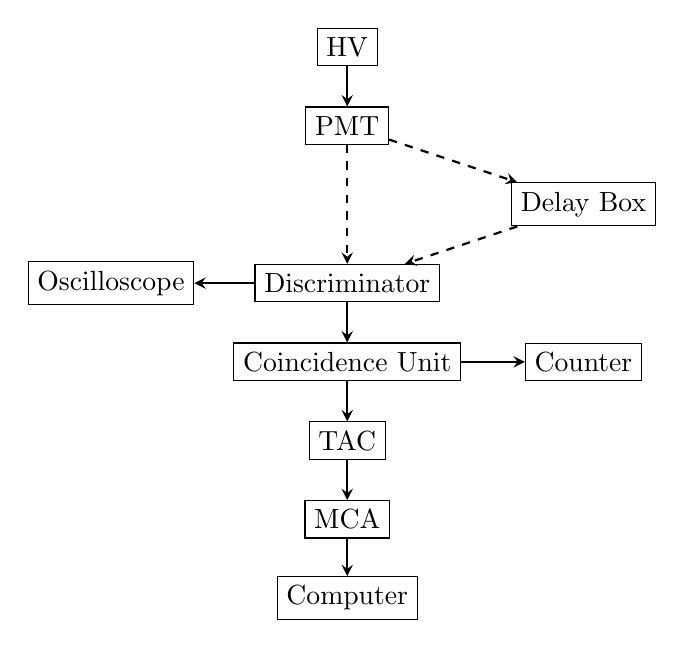
\begin{tikzpicture}[node distance=.3cm]
      %http://www.texample.net/tikz/examples/feature/arrows/
      \usetikzlibrary{shapes.geometric, arrows} 
      \tikzstyle{startstop} = [rectangle, rounded corners, minimum width=.2cm, minimum height=.2cm,text centered, draw=black]
      \tikzstyle{rect} = [rectangle, minimum width=.2cm, minimum height=.2cm, text centered, draw=black]%, fill=orange!30]
      \tikzstyle{parallelogram} = [diamond, minimum width=.2cm, minimum height=.2cm, text centered,draw=black]
      \tikzstyle{arrow} = [thick,->,>=stealth]
      \node (Aname) at (-3,4) [rect] {HV};
      \node (Bname) at (-3,3) [rect] {PMT};
      \node (Cname) at (0,2) [rect] {Delay Box};
      \node (Dname) at (-3,1) [rect] {Discriminator};
      \node (Ename) at (-6,1) [rect] {Oscilloscope};
      \node (Fname) at (-3,0) [rect] {Coincidence Unit};
      \node (Gname) at (0,0) [rect] {Counter};
      \node (Hname) at (-3,-1) [rect] {TAC};
      \node (Iname) at (-3,-2) [rect] {MCA};
      \node (Jname) at (-3,-3) [rect] {Computer};

      \draw [arrow] (Aname) -- (Bname);
      \draw [dashed,arrow] (Bname) -- (Cname);
      \draw [dashed,arrow] (Cname) -- (Dname);
      \draw [dashed,arrow] (Bname) -- (Dname);
      \draw [arrow] (Dname) -- (Ename);
      \draw [arrow] (Dname) -- (Fname);
      \draw [arrow] (Fname) -- (Gname);
      \draw [arrow] (Fname) -- (Hname);
      \draw [arrow] (Hname) -- (Iname);
      \draw [arrow] (Iname) -- (Jname);
    \end{tikzpicture}
    \caption{\small{A schematic for the electronics included in the apparatus. Dashed line represent interchanging schemes for different procedures of the study. \label{scheme}}}
    %\caption{\small{Schematic of experimental apparatus. \label{fig:aparatuslatex}}}
    \end{center}
  \end{figure}

\begin{figure}[htb!]
  \begin{center}
\centerline{\includegraphics[width=1.5in]{appar.png}}
\caption{ \small{The detector set up with a diverse range of height separations between the PMTs. A)\,PMT A B)\,PMT B C)\,PMT C D)\,PMT D E)\,Cosmic Ray Muon}}
\label{appa}
  \end{center}
\end{figure}


\section{Procedure}


% you always need to end an environment { } you have started--just like in C

The four muon detectors were plateaued before any data collection was done. Detectors A, B, C, and D were calibrated at 1750\,V, 1550\,V, 1400\,V, and 1600\,V, respectively.
\\
\indent To measure the vertical muon flux, two detectors were gradually separated by defined heights. A set time interval was specified, and the counts were measured for each height identity. The solid angle, $\Omega$, was derived from equation\,\ref{sa} using measured parameters of the detectors. Equation\,\ref{sa} incorporated the area of the detectors, $\omega$, and the separation distance between the two detectors, h.
\\
\indent The prime directionality was determined by shifting the detectors {34.1\degree} from the zenith. The tilted detectors were then rotated to represent muon flux in the north, south, east, and west cardinal directions. 

\begin{equation}
\Omega=4\left[\arccos\left(  -\frac{\omega^2/4}{h^2+\omega^2/4}\right)  \right]-2\pi
\label{sa}
\end{equation}

\begin{equation}
\text{Vertical Muon Flux}=\frac{\text{Counts}}{\Omega}
\label{flux}
\end{equation}
\\
\indent The muon lifetime was found by triggering on muons that pass through the top two counters but stop in the large block of scintillator\,\cite{1}. The counting timer elapsed a total of 510840\,seconds or 5.91\,days. Any signal that passed through detector D in figure\,\ref{appa} were vetoed and rejected from counting. Before data collection, a calibration curve was generated from 0.5\,$\mu$s to 3.5\,$\mu$s against channel numbers of the Multi-Channel Analyzer\,(MCA)\,\cite{3}. Using the calibration and the measured flux of muons, the fit parameters of the resulting plot yielded the muon lifetime.




\section{Calculation of Results and Errors}

\subsection{Flux against Solid Angle and Spacing between Detectors}

\begin{figure}[h!]
  \begin{center}
\centerline{\includegraphics[width=3.5in]{vertsa2.pdf}}
\caption{ \small{Solid angle against counts with a linear relationship between the two proportionally increasing parameters. \label{figsa}}}
%  \end{center}
%\end{figure}
%
\vspace{.5 cm}
%
%\begin{figure}[h!]
%  \begin{center}
\centerline{\includegraphics[width=3.5in]{vertfd2.pdf}}
\caption{ \small{Muon vertical flux relationship between the solid angle, counts, and the separation between detectors. The flux is constant while increasing detector separation distance. \label{fig1}}}
  \end{center}
\end{figure}

The study infers that increased solid angles, $\Omega$, are proportional to increased counts. Figure\,\ref{figsa} shows the aforementioned statement as the counts proportionally increased with the escalated solid angles.
\\
\indent The muon vertical flux exhibited a converse behavior to the solid angle counts. Figure\,\ref{fig1} showed increasing detector separation versus the flux. Vertical muon flux was practically constant within the flux error, which showed that the relation between the flux and solid angle was independent of the separation distance. The resulting slope from the vertical flux was (-0.23$\pm$0.28)\,counts/sr/cm, which is consistent with zero within the error bars.


\subsection{Cardinal Direction}
\begin{figure}[h!]
  \begin{center}
\centerline{\includegraphics[width=3.5in]{direction2.pdf}}
\caption{ \small{A directionality map that illustrates the directional bias in the westward cardinal direction with approximately (708$\pm$27)\,counts. \label{cardinal}}}
  \end{center}
\end{figure}
\vspace{.1 mm}
Figure\,\ref{cardinal} showed that the muon directionality had an extreme westward bias of (708$\pm$27)\,counts. Conversely, the north, east, and southward flux were (641$\pm$25)\,counts, (639$\pm$25)\,counts, and (663$\pm$26)\,counts, respectively. The cardinal direction bias was attributed to the geomagnetic cutoff of the Earth's magnetic field, which allows only certain directions and rigidities of cosmic ray flux at equatorial latitudes.


\subsection{Muon Lifetime}

\begin{figure}[h!]
  \begin{center}
\centerline{\includegraphics[width=3.5in]{calib2.pdf}}
\caption{ \small{A calibration curve with a linear fit used to convert MCA channel numbers into respective and proportional time. \label{calibration}}}
  \end{center}
\end{figure}
\vfill\eject
The calibration curve in figure\,\ref{calibration} yielded a linear fit that included parameters to convert channel numbers into a time axis. The axis was converted from seconds to microseconds. The conversion parameters were used to manipulate the muon lifetime channel numbers into microseconds in figure\,\ref{life}.


\begin{figure}[h!]
  \begin{center}
\centerline{\includegraphics[width=3.5in]{muonlifetime2.pdf}}
\caption{ \small{Binned values of the muon lifetime portion of the study. A exponential fit is linearly placed to signify the regression as time elapses. \label{life}}}
  \end{center}
\end{figure}

\begin{table}[h!] 
\caption{ Experimental muon lifetime versus the actual lifetime}
    %table caption at the top is standard
\label{t1}   % labels are used to refer to this in the text
 \begin{center}   % center the table on the page
    \begin{tabular}{|c|c|c|c|} \hline   % tabular environment 
Counting  & Experimental & Actual Mean & Error \\
 Time   & Muon Lifetime & Muon Lifetime &  \\
 (days) & ($\mu$s)  & ($\mu$s) &   \\ \hline \hline \hline
5.91 & 2.26$\pm$0.16 & 2.20 & 0.38$\sigma$ \\ \hline
     \end{tabular}
  \end{center}
\end{table}

\begin{equation}
ae^{-t/\tau}=e^{p_0x+p_1}
\label{orig}
\end{equation}
\begin{equation}
-\frac{1}{p_0}=\tau
\label{derived}
\end{equation}

 Muon lifetime, $\tau$, was determined by the slope of the experiment in figure\,\ref{life}. As time elapsed, the number of muon decay decreased causing the regression originally in the MCA bins. The parameters of the slope were determined with an exponential fit, provided in equation\,\ref{orig}. A muon lifetime expression inverse to the slope, derived in equation\,\ref{derived}, resulted in an experimental muon lifetime of (2.26$\pm$0.16)\,$\mu$s. The actual mean lifetime of a muon is 2.20\,$\mu$s, therefore the experimental lifetime had a discrepancy of 0.38$\sigma$\,\cite{4}.


\clearpage
\section{Discussion and Conclusion}

This study determined a muon lifetime of (2.26$\pm$0.16)\,$\mu$s. A deviation of 0.38$\sigma$, from the literature value of 2.20\,$\mu$s, showed that the experiment was accurate in determining the lifetime of a muon. The vertical flux yielded a slope of (-0.23$\pm$0.28)\,{counts/sr/cm}, which was consistent with zero. This result showed that muon flux was independent of detector separation, but counts were primarily correlated to deviations in the solid angle. The study also showed the directional dependence of detected muon flux, with a significant westward bias of (708$\pm$27)\,counts.
\\
\indent The muon flux with solid angles exhibited the desired qualities, but there were large statistical errors when deriving the flux and solid angle ratio. Westward bias for muon flux was also accurate qualitatively, but the result was hindered as the southward cardinal direction is similar to the western flux within the error. The largest source of statistical error of calculations involved in this study were attributed to the Poisson error derived from the muon counts.
\vfill\eject

\section{Acknowledgments}
Special thanks to Christina Nelson for the idea of cosmic ray significance and the illustration of cosmic ray air showers. Figure\,\ref{scheme} was generated by authors Daichi Hiramatsu and Corey Mutnik, and was included within the study.

% the following \setlength is to force the bibliography to have no
% paragraph indentations.Can use vairous units--cm are used here.
\setlength{\parindent}{0cm}

\begin{thebibliography}{99}  % the trailing 99 controls some obscure format--just use

\bibitem{1} \url{http://www.phys.hawaii.edu/~shige/phys481L/MuonDecay.txt}    % {\em } for emphasis, \textbf{ } for boldface

\bibitem{2} \url{http://www.geek.com/wp-content/uploads/2014/10/cosmicrays2.jpg}

\bibitem{3} "Multichannel Analyzer (MCA) Application Software." Nuclear Applications Software|ORTEC Scientific Equipment. ORTEC. Web. 5 Nov. 2015.

\bibitem{4} \url{http://pdg.lbl.gov/2012/tables/rpp2012-sum-leptons.pdf}




\end{thebibliography}





\end{document}

